\documentclass[8pt]{extarticle}
\title{}
\author{Avinash Iyer}
\date{}
\usepackage[shortlabels]{enumitem}

%font setup
%
\usepackage{newpxtext,eulerpx}

%paper setup
\usepackage{geometry}
\geometry{letterpaper, portrait, margin=1in}
\usepackage{fancyhdr}

%symbols
\usepackage{amsmath}
\usepackage{mathtools}
\usepackage{hyperref}
\usepackage{gensymb}

\usepackage[T1]{fontenc}
\usepackage[utf8]{inputenc}

%chemistry stuff
\usepackage[version=4]{mhchem}
\usepackage{chemfig}

%plotting
\usepackage{pgfplots}
\usepackage{tikz}
\tikzset{middleweight/.style={pos = 0.5, fill=white}}
\tikzset{weight/.style={pos = 0.5, fill = white}}
\tikzset{lateweight/.style={pos = 0.75, fill = white}}
\tikzset{earlyweight/.style={pos = 0.25, fill=white}}

%\usepackage{natbib}

%graphics stuff
\usepackage{graphicx}
\graphicspath{ {./images/} }

%code stuff
%when using minted, make sure to add the -shell-escape flag
%you can use lstlisting if you don't want to use minted
%\usepackage{minted}
%\usemintedstyle{pastie}
%\newminted[javacode]{java}{frame=lines,framesep=2mm,linenos=true,fontsize=\footnotesize,tabsize=3,autogobble,}
%\newminted[cppcode]{cpp}{frame=lines,framesep=2mm,linenos=true,fontsize=\footnotesize,tabsize=3,autogobble,}

\usepackage{listings}
\usepackage{color}
\definecolor{dkgreen}{rgb}{0,0.6,0}
\definecolor{gray}{rgb}{0.5,0.5,0.5}
\definecolor{mauve}{rgb}{0.58,0,0.82}

\lstset{frame=tb,
	language=Java,
	aboveskip=3mm,
	belowskip=3mm,
	showstringspaces=false,
	columns=flexible,
	basicstyle={\small\ttfamily},
	numbers=none,
	numberstyle=\tiny\color{gray},
	keywordstyle=\color{blue},
	commentstyle=\color{dkgreen},
	stringstyle=\color{mauve},
	breaklines=true,
	breakatwhitespace=true,
	tabsize=3
}
% text + color boxes
\usepackage{tcolorbox}
\tcbuselibrary{breakable}
\newtcolorbox{problem}[1]{colback = white, title = {#1}, breakable}
\newtcolorbox{solution}{colback = white, colframe = black!75!white, title = Solution, breakable}
%including PDFs
\usepackage{pdfpages}
\setlength{\parindent}{0pt}

\pagestyle{fancy}
\fancyhf{}
\rhead{Avinash Iyer}
\lhead{Math 400: Class Notes}
\begin{document}{
  \begin{problem}{Graphs and the Three Utilities Problem}
    We can imagine trying to connect three houses below with three utilities without the utility lines crossing.
    \begin{center}
      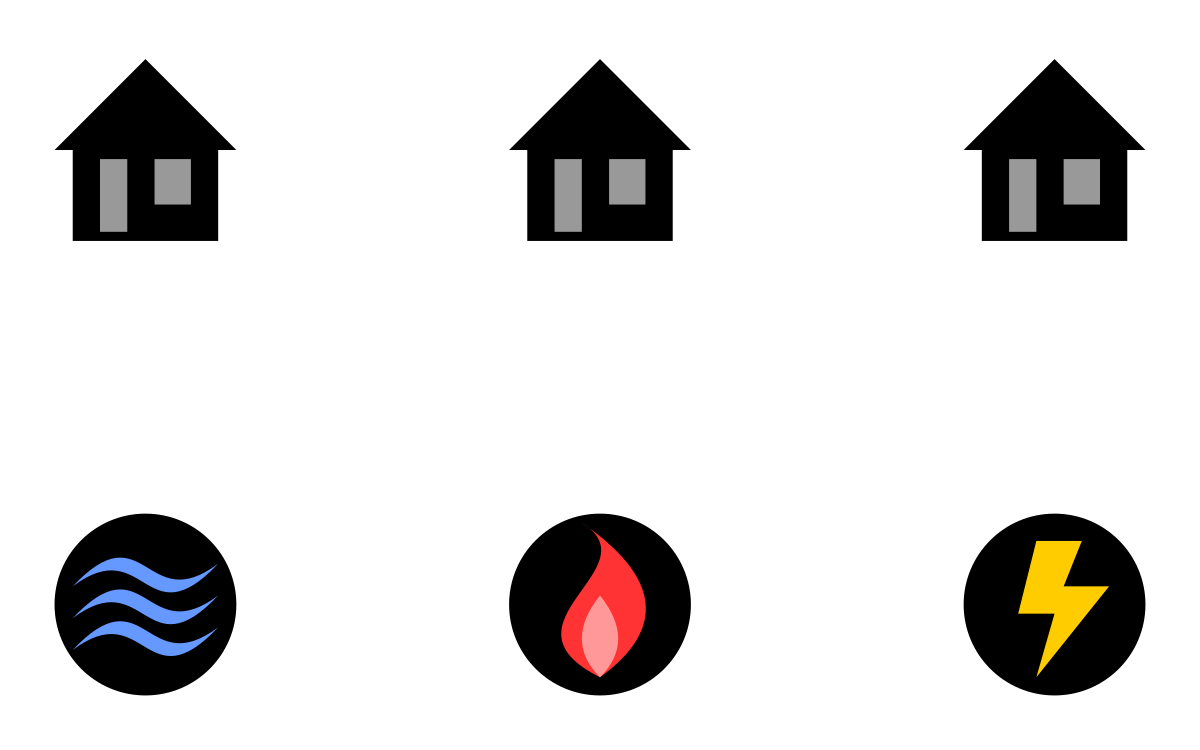
\includegraphics[width=10cm]{3_utilities_problem_blank}
    \end{center}
    This problem is akin to the graph $K_{3,3}$ (the complete bipartite graph with three vertices in each partite set). 
    \begin{center}
      \begin{tikzpicture}
        \filldraw (-1,0) circle (2pt)
              (-1,1) circle (2pt)
              (-1,-1) circle (2pt)
              (1,0) circle (2pt)
              (1,1) circle (2pt)
              (1,-1) circle (2pt);
        \draw (-1,0) -- (1,0) -- (-1,1) -- (1,1) -- (-1,-1) -- (1,-1) -- (-1,0);
        \draw (1,-1) -- (-1,1);
        \draw (1,1) -- (-1,0);
        \draw (1,0) -- (-1,-1);
      \end{tikzpicture}
    \end{center}
    A \textit{graph} is an ordered pair of sets $(V,E)$, where $E\subseteq V\times V$.\\

    For example, if $V = \{a,b,c\}$ and $E = \{(a,b),(a,c)\}$, then $(V,E)$ is a graph. The goal of the three utilities puzzle is to draw $K_{3,3}$ in $\mathbb{R}^2$ without any edges crossing. A graph that can be drawn as such is \textit{planar}.
    \begin{itemize}
      \item $K_{3,3}$ is not planar.
      \item $K_{2,4}$ is planar.
    \end{itemize}
    \begin{center}
      \begin{tikzpicture}
        \filldraw (-2,0) circle (2pt)
                  (2,0) circle (2pt)
                  (0,0.5) circle (2pt)
                  (0,1.5) circle (2pt)
                  (0,-0.5) circle (2pt)
                  (0,-1.5) circle (2pt);
        \draw (-2,0) -- (0,1.5);
        \draw (-2,0) -- (0,-1.5);
        \draw (-2,0) -- (0,0.5);
        \draw (-2,0) -- (0,-0.5);
        \draw (2,0) -- (0,1.5);
        \draw (2,0) -- (0,-1.5);
        \draw (2,0) -- (0,0.5);
        \draw (2,0) -- (0,-0.5);
      \end{tikzpicture}
    \end{center}
    \begin{problem}{Euler's Theorem}
      Let $G\subseteq \mathbb{R}^2$ be a planar graph (i.e., drawn in $\mathbb{R}^2$ without edge crossings). Each disjoint subset of $\mathbb{R}^2-G$ is a \textit{face} of G.\\

      For every graph $G$ embedded in $\mathbb{R}^2$ (i.e., drawn without edge crossings) with $V$ vertices, $E$ edges, and $F$ faces, the following is true:
      \[
        V-E+F = 2
      \]
    \end{problem}
    We will use this theorem to show that you cannot connect the three houses to the three utilities as follows:
    \begin{problem}{Outline Proof (of $K_{3,3}$'s non-planarity)}
      Suppose toward contradiction that $K_{3,3}$ is planar. Then, by Euler's Theorem, we know that $V-E+F = 2$.\\

      We know that $K_{3,3}$ has six vertices and nine edges, so we know that $6-9+F = 2$. Therefore, we know that there must be $5$ faces. In order to enclose a face, there must be at least four edges in $K_{3,3}$ (as there is no edge between two members of a partite set). Additionally, each edge encloses two faces. Therefore, $E\geq 2F$. However, since $E = 9$, and we assume that $F\geq 5$, we have reached a contradiction (as $9<10$). Thus, $K_{3,3}$ is not planar.
    \end{problem}
    \begin{problem}{Four-Color Theorem}
      Every planar graph can be colored (adjacent vertices do not have the same color) with four colors. The planar graph can be colored by fewer colors.
    \end{problem}
    \begin{problem}{Polynomial Example}
      Let $p(a,b,c,d) = ab + ac + ad + bc +bd + cd$. When we factor, we get $p(a,b,c,d) = a(b+c+d) + b(c+d) + cd$. In the first equation, we had to carry out 6 multiplications, while in the second equation we only had to carry out 3 multiplications. We could factor differently:
      \begin{align*}
        p(a,b,c,d) &= ab + ac + ad + bc + bd + cd \\
                   &= a(b+c+d) + b(c+d) + cd\\
                   &= (a+b)(c+d) + ab + cd
      \end{align*}
      We have a lower bound of three multiplications to carry out.\\

      In the arbitrary case, we have the following. We want to find the lowest number of multiplications.
      \begin{align*}
        p(x_1,\dots,x_n) &= \sum_{i = 1}^{n-1}\sum_{j = i+1}^{n} x_ix_j
      \end{align*}
      \tcblower
      The minimum number of multiplications we can do is $n-1$. We can find this via a graph with $n$ vertices $\{x_1,\dots,x_n\}$, and for $x_ix_j$ in $p$, we have an edge from $x_i$ to $x_j$. This is the complete graph on $n$ vertices, $K_n$. Each complete bipartite subgraph represents a multiplication — so our question can be restated as follows:
      \begin{quote}
          Given a complete graph on $n$ vertices, $K_n$, partition its edges into as few complete graphs as possible.
      \end{quote}
      The answer for this is $n-1$, with a proof in linear algebra. However, there is no graph theory-specific proof for this question.
    \end{problem}
  \end{problem}
}\end{document}
